\lab{Matplotlib Syntax and Customization Guide}{Matplotlib Customization}

\objective{
The documentation for Matplotlib can be a little difficult to maneuver and basic information is sometimes difficult to find.
This appendix condenses and demonstrates some of the more applicable and useful information on plot customizations.
It is not intended to be read all at once, but rather to be used as a reference when needed.
For an interative introduction to Matplotlib, see the Introduction to Matplotlib lab in Python Essentials.
For more details on any specific function, refer to the Matplotlib documentation at \url{https://matplotlib.org/}.
}

\section*{Matplotlib Interface} %==================================
%This section is largely taken from MatplotlibIntro. I'm unsure about how important this part is.
Matplotlib plots are made in a \li{Figure} object that contains one or more \li{Axes}, which themselves contain the graphical plotting data.
Matplotlib provides two ways to create plots:
\begin{enumerate}
\item Call plotting functions directly from the module, such as \li{plt.plot()}.
This will create the plot on whichever \li{Axes} is currently active.
\item Call plotting functions from an \li{Axes} object, such as \li{ax.plot()}.
This is particularly useful for complicated plots and for animations.
\end{enumerate}

Table \ref{mpl:interface} contains a summary of functions that are used for managing \li{Figure} and \li{Axes} objects.

\begin{table}[H]
\centering
\begin{tabular}{r|l}
    Function & Description\\
    \hline
    \li{add_subplot()} & Add a single subplot to the current figure\\
    \li{axes()} & Add an axes to the current figure\\
    \li{clf()} & Clear the current figure\\
    \li{figure()} & Create a new figure or grab an existing figure\\
    \li{gca()} & Get the current axes\\
    \li{gcf()} & Get the current figure\\
    %\li{ion()} & Turn on interactive mode\\
    %\li{iof()} & Turn off interactive mode\\
    \li{subplot()} & Add a single subplot to the current figure\\
    \li{subplots()} & Create a figure and add several subplots to it\\
\end{tabular}
\caption{Basic functions for managing plots.}
\label{mpl:interface}
\end{table}

\li{Axes} objects are usually managed through the functions \li{plt.subplot()} and \li{plt.subplots()}.
The function \li{subplot()} is used as \li{plt.subplot(nrows, ncols, plot_number)}.
Note that if the inputs for \li{plt.subplot()} are all integers, the commas between the entries can be omitted.
For example, \li{plt.subplot(3,2,2)} can be shortened to \li{plt.subplot(322)}.
%This both returns that subplot and sets it as the active one.

The function \li{subplots()} is used as \li{plt.subplots(nrows, ncols)}, and returns a \li{Figure} object and an array of \li{Axes}.
This array has the shape \li{(nrows, ncols)}, and can be accessed as any other array.
Figure \ref{mpl:subplots-layout} demonstrates the layout and indexing of subplots.

\begin{figure}[H] % The layout created by subplots(23i).
%Taken from matplotlib intro
\captionsetup[subfigure]{justification=centering}
\centering
\begin{framed}
\begin{subfigure}{.32\textwidth}
    \centering
    
\includegraphics[width=\linewidth]{figures/layout_1.pdf}
\end{subfigure}
%
\begin{subfigure}{.32\textwidth}
    \centering
    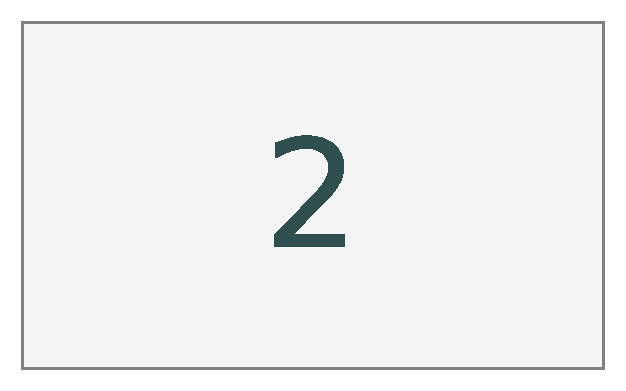
\includegraphics[width=\linewidth]{figures/layout_2.pdf}
\end{subfigure}
%
\begin{subfigure}{.32\textwidth}
    \centering
    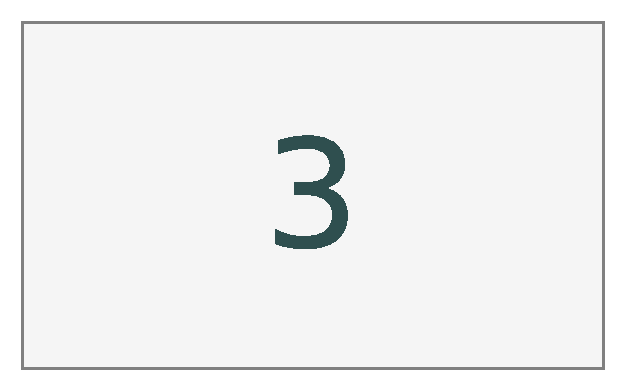
\includegraphics[width=\linewidth]{figures/layout_3.pdf}
\end{subfigure}
\\
\begin{subfigure}{.32\textwidth}
    \centering
    
\includegraphics[width=\linewidth]{figures/layout_4.pdf}
\end{subfigure}
%
\begin{subfigure}{.32\textwidth}
    \centering
    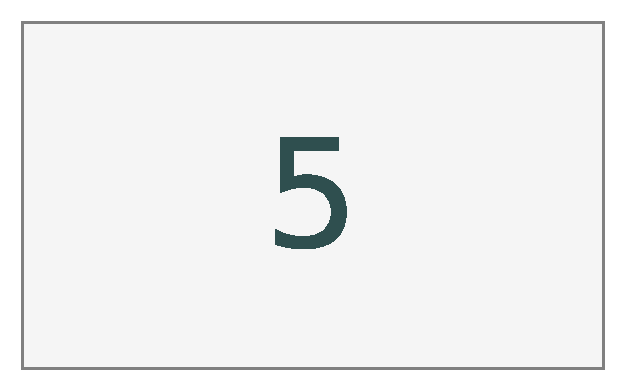
\includegraphics[width=\linewidth]{figures/layout_5.pdf}
\end{subfigure}
%
\begin{subfigure}{.32\textwidth}
    \centering
    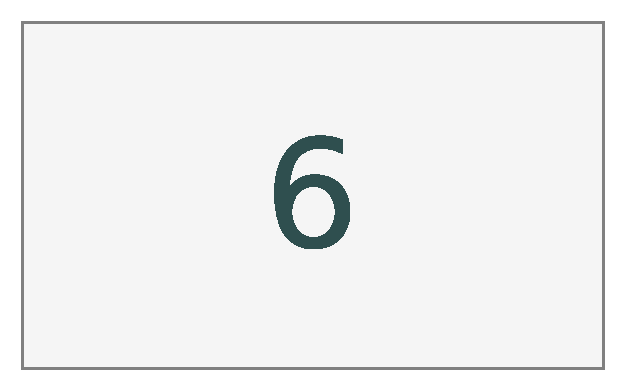
\includegraphics[width=\linewidth]{figures/layout_6.pdf}
\end{subfigure}
\end{framed}
\caption{The layout of subplots with \li{plt.subplot(2,3,i)} (2 rows, 3 columns), where \li{i} is the index pictured above. The outer border is the figure that the axes belong to.}
\label{mpl:subplots-layout}
\end{figure}

The following example demonstrates three equivalent ways of producing a figure with two subplots, arranged next to each other in one row:
\begin{lstlisting}
>>> x = np.linspace(-5, 5, 100)

# 1. Use plt.subplot() to switch the current axes.
>>> plt.subplot(121)
>>> plt.plot(x, 2*x)
>>> plt.subplot(122)
>>> plt.plot(x, x**2)

# 2. Use plt.subplot() to explicitly grab the two subplot axes.
>>> ax1 = plt.subplot(121)
>>> ax1.plot(x, 2*x)
>>> ax2 = plt.subplot(122)
>>> ax2.plot(x, x**2)

# 3. Use plt.subplots() to get the figure and all subplots simultaneously.
>>> fig, axes = plt.subplots(1, 2)
>>> axes[0].plot(x, 2*x)
>>> axes[1].plot(x, x**2)
\end{lstlisting}

\begin{warn}
Be careful not to mix up the following similarly-named functions:
\begin{enumerate}
    \item \li{plt.axes()} creates a new place to draw on the figure, while \li{plt.axis()} or \li{ax.axis()} sets properties of the $x$- and $y$-axis in the current axes, such as the $x$ and $y$ limits.
    \item \li{plt.subplot()} (singular) returns a single subplot belonging to the current figure, while \li{plt.subplots()} (plural) creates a new figure and adds a collection of subplots to it.
\end{enumerate}
\end{warn}

\section*{Plot Customization} %=====================================

\subsection*{Styles}%=====================================
Matplotlib has a number of built-in styles that can be used to set the default appearance of plots.
These can be used via the function \li{plt.style.use()}; for instance, \li{plt.style.use("seaborn")} will have Matplotlib use the "seaborn" style for all plots created afterwards.
A list of built-in styles can be found at \url{https://matplotlib.org/stable/gallery/style_sheets/style_sheets_reference.html}.

The style can also be changed only temporarily using \li{plt.style.context()} along with a \li{with} block:
\begin{lstlisting}
with plt.style.context('dark_background'):
    # Any plots created here use the new style
    plt.subplot(1,2,1)
    plt.plot(x, y)
    # ...
# Plots created here are unaffected
plt.subplot(1,2,2)
plt.plot(x, y)
\end{lstlisting}

\subsection*{Plot layout} %=====================================
\subsubsection*{Axis properties} %================================
Table \ref{mpl:axis} gives an overview of some of the functions that may be used to configure the axes of a plot.

\begin{table}%[H] %better for fitting stuff in pages
\centering
\begin{tabular}{r|l}
    Function & Description\\
    \hline
    \li{axis()} & set the $x$- and $y$-limits of the plot\\
    \li{grid()} & add gridlines\\
    \li{xlim()} & set the limits of the $x$-axis\\
    \li{ylim()} & set the limits of the $y$-axis\\
    \li{xticks()} & set the location of the tick marks on the $x$-axis\\
    \li{yticks()} & set the location of the tick marks on the $y$-axis\\
    \li{xscale()} & set the scale type to use on the $x$-axis\\
    \li{yscale()} & set the scale type to use on the $y$-axis\\
    \li{ax.spines[side].set_position()} & set the location of the given spine\\
    \li{ax.spines[side].set_color()} & set the color of the given spine\\
    \li{ax.spines[side].set_visible()} & set whether a spine is visible\\
    %\li{ax.xaxis}/\li{yaxis.set_ticks_position()} & set the position of the tick marks on the given axis\\
\end{tabular}
\caption{Some functions for changing axis properties. \li{ax} is an \li{Axes} object.}
\label{mpl:axis}
\end{table}

The functions \li{xlim()}, \li{ylim()}, and \li{axis()} are used to set one or both of the x and y ranges of the plot.
\li{xlim()} and \li{ylim()} each accept two arguments, the lower and upper bounds, or a single list of those two numbers.
\li{axis()} accepts a single list consisting, in order, of \li{xmin, xmax, ymin, ymax}.
Passing \li{None} instead of one of the numbers to any of these functions will make it not change the corresponding value from what it was.
Each of these functions can also be called without any arguments, in which case it will return the current bounds.
Note that \li{axis()} can also be called directly on an \li{Axes} object, while \li{xlim()} and \li{ylim()} cannot.

\li{axis()} also can be called with a string as its argument, which has several options.
The most common is \li{axis('equal')}, which makes the scale of the x- and y-scales equal (i.e. makes circles circular).

To use a logarithmic scale on an axis, the functions \li{xscale("log")} and \li{yscale("log")} can be used.
%There are several other scale types available, although used less frequenlty: \li{"linear"}, which creates a linear scale; \li{"symlog"}, which uses a logarithmic scale for both positive and negative values; and \li{"logit"}, which is based off of the logistic function.

The functions \li{xticks()} and \li{yticks()} accept a list of tick positions, which the ticks on the corresponding axis are set to.
Generally, this works the best when used with \li{np.linspace()}.
This function also optionally accepts a second argument of a list of labels for the ticks.
If called with no arguments, the function returns a list of the current tick positions and labels instead.

The spines of a Matplotlib plot are the black border lines around the plot, with the left and bottom ones also being used as the axis lines.
To access the spines of a plot, call \li{ax.spines[side]}, where \li{ax} is an \li{Axes} object and \li{side} is \li{'top'}, \li{'bottom'}, \li{'left'}, or \li{'right'}.
Then, functions can be called on the \li{Spine} object to configure it.

The function \li{spine.set_position()} has several ways to specify the position.
The two simplest are with the arguments \li{'center'} and \li{'zero'}, which place the spine in the center of the subplot or at an x- or y-coordinate of zero, respectively.
The others are a passed as a tuple \li{(position\_type, amount)}:
\begin{itemize}
\item \li{'data'}: place the spine at an x- or y-coordinate equal to \li{amount}.
\item \li{'axes'}: place the spine at the specified \li{Axes} coordinate, where 0 corresponds to the bottom or left of the subplot, and 1 corresponds to the top or right edge of the subplot.
\item \li{'outward'}: places the spine \li{amount} pixels outward from the edge of the plot area.
A negative value can be used to move it inwards instead.
\end{itemize}

\li{spine.set_color()} accepts any of the color formats Matplotlib supports.
Alternately, using \li{set_color('none')} will make the spine not be visible.
\li{spine.set_visible()} can also be used for this purpose.

The following example adjusts the ticks and spine positions to improve the readability of a plot of $\sin(x)$. The result is shown in Figure \ref{mpl:spines}.
\begin{lstlisting}
>>> x = np.linspace(0,2*np.pi,150)
>>> plt.plot(x, np.sin(x))
>>> plt.title(r"$y=\sin(x)$")

#Set the ticks to multiples of pi/2, make nice labels
>>> ticks = np.pi / 2 * np.array([0,1,2,3,4])
>>> tick_labels = ["$0$", r"$\frac{\pi}{2}$", r"$\pi$", r"$\frac{3\pi}{2}$",
...                 r"$2\pi$"]
>>> plt.xticks(ticks, tick_labels)

#Move the bottom spine to zero, remove the top and right ones
>>> ax = plt.gca()
>>> ax.spines['bottom'].set_position('zero')
>>> ax.spines['right'].set_color('none')
>>> ax.spines['top'].set_color('none')

>>> plt.show()
\end{lstlisting}
\begin{figure}[H]
\centering
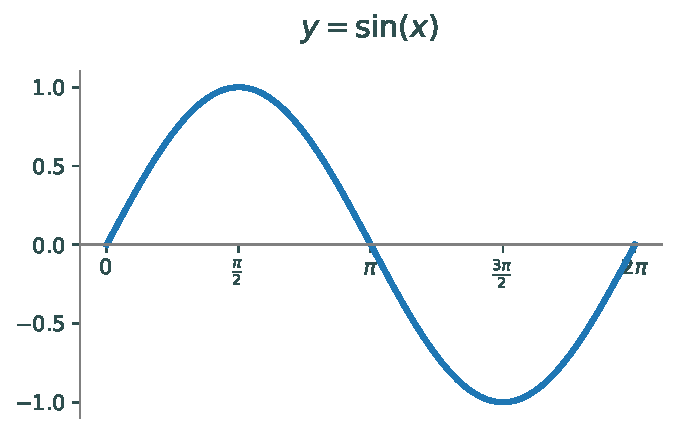
\includegraphics[width=4in]{figures/axis_example.pdf}
\caption{Plot of $y=\sin(x)$ with axes modified for clarity}
\label{mpl:spines}
\end{figure}

\subsubsection*{Plot Layout} %===================================
The position and spacing of all subplots within a figure can be modified using the function \li{plt.subplots_adjust()}.
This function accepts up to six keyword arguments that change different aspects of the spacing.
\li{left}, \li{right}, \li{top}, and \li{bottom} are used to adjust the rectangle around all of the subplots.
In the coordinates used, 0 corresponds to the bottom or left edge of the figure, and 1 corresponds to the top or right edge of the figure.
\li{hspace} and \li{wspace} set the vertical and horizontal spacing, respectively, between subplots.
The units for these are in fractions of the average height and width of all subplots in the figure.
%
If more fine control is desired, the position of individual \li{Axes} objects can also be changed using \li{ax.get_position()} and \li{ax.set_position()}.
%Possibly too much info; can be learned from experimentation/documentation
%Note that \li{ax.get_position()} returns a Matplotlib \li{Bbox} (bounding box) object; the left, right, bottom, and top edges are accessed as \li{box.x0}, \li{box.x1}, \li{box.y0}, and \li{box.y1}, respectively.
%\li{ax.set_position()} accepts either a \li{Bbox} object or a list consisting of \li{[left, bottom, width, height]}.
%All of these positions are all specified in terms of the whole figure, with (0,0) being the bottom-left and (1,1) being the top-right.

The size of the figure can be configured using the \li{figsize} argument when creating a figure:
\begin{lstlisting}
>>> plt.figure(figsize=(12,8))
\end{lstlisting}
Note that many environments will scale the figure to fill the available space.
Even so, changing the figure size can still be used to change the aspect ratio as well as the relative size of plot elements.

The following example uses \li{subplots_adjust()} to create space for a legend outside of the plotting space. The result is shown in Figure \ref{mpl:positioning}.
\begin{lstlisting}
#Generate data
>>> x1 = np.random.normal(-1, 1.0, size=60)
>>> y1 = np.random.normal(-1, 1.5, size=60)
>>> x2 = np.random.normal(2.0, 1.0, size=60)
>>> y2 = np.random.normal(-1.5, 1.5, size=60)
>>> x3 = np.random.normal(0.5, 1.5, size=60)
>>> y3 = np.random.normal(2.5, 1.5, size=60)

#Make the figure wider
>>> fig = plt.figure(figsize=(5,3))

#Plot the data
>>> plt.plot(x1, y1, 'r.', label="Dataset 1")
>>> plt.plot(x2, y2, 'g.', label="Dataset 2")
>>> plt.plot(x3, y3, 'b.', label="Dataset 3")

#Create a legend to the left of the plot
>>> lspace = 0.35
>>> plt.subplots_adjust(left=lspace)
#Put the legend at the left edge of the figure
>>> plt.legend(loc=(-lspace/(1-lspace),0.6))
>>> plt.show()
\end{lstlisting}
\begin{figure}[H]
\centering
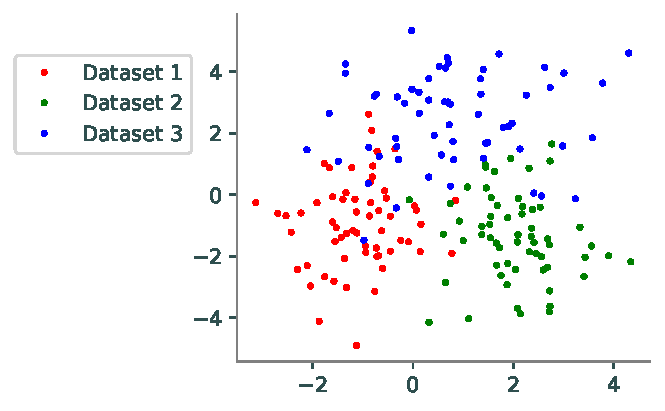
\includegraphics[width=4in]{figures/positioning_example.pdf}
\caption{Example of repositioning axes.}
\label{mpl:positioning}
\end{figure}

\subsection*{Colors} %========================================
The color that a plotting function uses is specified by either the \li{c} or \li{color} keyword arguments; for most functions, these can be used interchangeably.
There are many ways to specific colors.
The most simple is to use one of the basic colors, listed in Table \ref{mpl:colors}.
Colors can also be specified using an RGB tuple such as \li{(0.0, 0.4, 1.0)}, a hex string such as \li{"0000FF"}, or a CSS color name like \li{"DarkOliveGreen"} or \li{"FireBrick"}.
A full list of named colors that Matplotlib supports can be found at \url{https://matplotlib.org/stable/gallery/color/named_colors.html}.
If no color is specified for a plot, Matplotlib automatically assigns it one from the default color cycle.

\begin{table}[H] % Basic colors.
\begin{tabular}{r|l}
    Code & Color \\
    \hline
    \li{'b'} & blue\\
    \li{'g'} & green\\
    \li{'r'} & red\\
    \li{'c'} & cyan\\
    \li{'m'} & magenta\\
\end{tabular}
\qquad
\begin{tabular}{r|l}
    Code & Color \\
    \hline
    \li{'y'} & yellow\\
    \li{'k'} & black\\
    \li{'w'} & white\\
    \li{'C0'} - \li{'C9'} & Default colors
\end{tabular}
\caption{Basic colors available in Matplotlib}
\label{mpl:colors}
\end{table}

Plotting functions also accept an \li{alpha} keyword argument, which can be used to set the transparency. A value of \li{1.0} corresponds to fully opaque, and \li{0.0} corresponds to fully transparent.

The following example demonstrates different ways of specifying colors:
\begin{lstlisting}
#Using a basic color
>>> plt.plot(x, y, 'r')
#Using a hexadecimal string
>>> plt.plot(x, y, color='FF0080')
#Using an RGB tuple
>>> plt.plot(x, y, color=(1, 0.5, 0))
#Using a named color
>>> plt.plot(x, y, color='navy')
\end{lstlisting}

\subsubsection*{Colormaps}
Certain plotting functions, such as heatmaps and contour plots, accept a colormap rather than a single color.
A full list of colormaps available in Matplotlib can be found at \url{https://matplotlib.org/stable/gallery/color/colormap_reference.html}.
Some of the more commonly used ones are \li{"viridis"}, \li{"magma"}, and \li{"coolwarm"}.
A colorbar can be added by calling \li{plt.colorbar()} after creating the plot.

Sometimes, using a logarithmic scale for the coloring is more informative.
To do this, pass a \li{matplotlib.colors.LogNorm} object as the \li{norm} keyword argument:
\begin{lstlisting}
# Create a heatmap with logarithmic color scaling
>>> from matplotlib.colors import LogNorm
>>> plt.pcolormesh(X, Y, Z, cmap='viridis', norm=LogNorm())
\end{lstlisting}


\subsection*{Text and Annotations} %========================================
Matplotlib has several ways to add text and other annotations to a plot, some of which are listed in Table \ref{mpl:text}.
The color and size of the text in most of these functions can be adjusted with the \li{color} and \li{fontsize} keyword arguments.

\begin{table}%[H] %makes the layout better
\centering
\begin{tabular}{r|l|l}
    Function & Description & Usage\\
    \hline
    \li{annotate()} & adds a commentary at a given point on the plot & annotate('text',(x,y))\\
    \li{arrow()} & draws an arrow from a given point on the plot & arrow(x,y,dx,dy)\\
    %\li{axhline()} & draws a horizontal line at y from xmin to xmax & axhline(y=0, xmin=0, xmax=1)\\
    %\li{axvline()} & draws a vertical line at x from ymin to ymax & axvline(x=0, ymin=0, ymax=1)\\
    %\li{axhspan()} & draws a rectangle from xmin to xmax across the plot & axhspan(ymin, ymax, xmin=0, xmax=1)\\
    %\li{axvspan()} & draws a rectangle from ymin to ymax across the plot & axvspan(xmin, xmax, ymin=0, ymin=1)\\
    \li{colorbar()} & Create a colorbar & colorbar()\\
    \li{legend()} & Place a legend in the plot & legend(loc='best')\\
    \li{text()} & Add text at a given position on the plot & text(x,y,'text')\\
    \li{title()} & Add a title to the plot & title('text')\\
    \li{suptitle()} & Add a title to the figure & suptitle('text')\\
    % \li{xticks()} & set the location of the tick marks on the x axis, returns current locations if no arguments are given\\
    % \li{yticks()} & set the location of the tick marks on the y axis, returns current locations if no arguments are given\\
    \li{xlabel()} & Add a label to the $x$-axis & xlabel('text') \\
    \li{ylabel()} & Add a label to the $y$-axis & ylabel('text')
\end{tabular}
\caption{Text and annotation functions in Matplotlib}
\label{mpl:text}
\end{table}

%From DataVisualization
Matplotlib also supports formatting text with \LaTeX, a system for creating technical documents.%
\footnote{See \url{http://www.latex-project.org/} for more information.}
To do so, use an \li{r} before the string quotation mark and surround the text with dollar signs.
This is particularly useful when the text contains a mathematical expression.
For example, the following line of code will make the title of the plot be $\frac{1}{2}\sin(x^2)$:
\begin{lstlisting}
>>> plt.title(r"$\frac{1}{2}\sin(x^2)$")
\end{lstlisting}

The function \li{legend()} can be used to add a legend to a plot.
Its optional \li{loc} keyword argument specifies where to place the legend within the subplot.
It defaults to \li{'best'}, which will cause Matplotlib to place it in whichever location overlaps with the fewest drawn objects.
The other locations this function accepts are \li{'upper right'}, \li{'upper left'}, \li{'lower left'}, \li{'lower right'}, \li{'center left'}, \li{'center right'}, \li{'lower center'}, \li{'upper center'}, and \li{'center'}.
Alternately, a tuple of \li{(x,y)} can be passed as this argument, and the bottom-left corner of the legend will be placed at that location.
The point (0,0) corresponds to the bottom-left of the current subplot, and (1,1) corresponds to the top-right.
This can be used to place the legend outside of the subplot, although care should be taken that it does not go outside the figure, which may require manually repositioning the subplots.

The labels the legend uses for each curve or scatterplot are specified with the \li{label} keyword argument when plotting the object.
Note that \li{legend()} can also be called with non-keyword arguments to set the labels, although it is less confusing to set them when plotting.

The following example demonstrates creating a legend:
\begin{lstlisting}
>>> x = np.linspace(0,2*np.pi,250)

# Plot sin(x), cos(x), and -sin(x)
# The label argument will be used as its label in the legend.
>>> plt.plot(x, np.sin(x), 'r', label=r'$\sin(x)$')
>>> plt.plot(x, np.cos(x), 'g', label=r'$\cos(x)$')
>>> plt.plot(x, -np.sin(x), 'b', label=r'$-\sin(x)$')

# Create the legend
>>> plt.legend()
\end{lstlisting}

\begin{comment} %More information than needed
The functions \li{text()}, \li{arrow()}, and \li{annotate()} each place the text or arrow at the specified location in data coordinates.
With \li{arrow()}, the properties of the arrow can be configured with the \li{width}, \li{head\_width}, \li{head\_length}, and \li{overhang} parameters. 
\li{annotate()} can also be used to create both an arrow and text, although it requires two more keyword arguments: \li{xytext}, which is a tuple specifying the text location; and \li{arrowprops}, which is a dictionary containing parameters for the arrow.
For example, the following code creates an arrow from (0,0) to (0.5,0.5) using \li{annotate()}: %
\footnote{This example is taken from \url{https://matplotlib.org/stable/api/_as_gen/matplotlib.pyplot.arrow.html}.}
\begin{lstlisting} 
>>> ax.annotate("", xy=(0.5, 0.5), xytext=(0, 0),
...             arrowprops={arrowstyle:"->"})
\end{lstlisting}
\end{comment}

\subsection*{Line and marker styles}
Matplotlib supports a large number of line and marker styles for line and scatter plots, which are listed in Table \ref{mpl:table-lmstyles}.
\begin{table}[H] % Line style
%\label{mpl:table-lmstyles} 
\centering
\begin{tabular}{c|l}
    character & description \\
    \hline
    - & solid line style \\
    -{}- & dashed line style\\
    -. & dash-dot line style \\
    : & dotted line style \\
    . & point marker \\
    , & pixel marker \\
    o & circle marker \\
    v & triangle\_down marker \\
    \^{} & triangle\_up marker \\
    $<$ & triangle\_left marker \\
    $>$ & triangle\_right marker \\
    1 & tri\_down marker \\
    2 & tri\_up marker \\
\end{tabular}
	\quad
\begin{tabular}{c|l}
    character & description \\
    \hline
    3 & tri\_left marker \\
    4 & tri\_right marker \\
    s & square marker \\
    p & pentagon marker \\
    * & star marker \\
    h & hexagon1 marker \\
    H & hexagon2 marker \\
    + & plus marker \\
    x & x marker \\
    D & diamond marker \\
    d & thin\_diamond marker \\
    $|$ & vline marker \\
    \_{} & hline marker \\
\end{tabular}
\caption{Available line and marker styles in Maplotlib.}
\label{mpl:table-lmstyles} 
\end{table}
The function \li{plot()} has several ways to specify this argument; the simplest is to pass it as the third positional argument.
The \li{marker} and \li{linestyle} keyword arguments can also be used.
The size of these can be modified using \li{markersize} and \li{linewidth}.
Note that by specifying a marker style but no line style, \li{plot()} can be used to make a scatter plot.
It is also possible to use both a marker style and a line style.
To set the marker using \li{scatter()}, use the \li{marker} keyword argument, with \li{s} being used to change the size.

The following code demonstrates specifying marker and line styles. The results are shown in Figure \ref{mpl:linestyles}.
\begin{lstlisting}
#Use dashed lines:
>>> plt.plot(x, y, '--')
#Use only dots:
>>> plt.plot(x, y, '.')
#Use dots with a normal line:
>>> plt.plot(x, y, '.-')
#scatter() uses the marker keyword:
>>> plt.scatter(x, y, marker='+')

#With plot(), the color to use can also be specified in the same string.
#Order usually doesn't matter.
#Use red dots:
>>> plt.plot(x, y, '.r')
#Equivalent:
>>> plt.plot(x, y, 'r.')

#To change the size:
>>> plt.plot(x, y, 'v-', linewidth=1, markersize=15)
>>> plt.scatter(x, y, marker='+', s=12)
\end{lstlisting}

\begin{figure}[H]
\centering
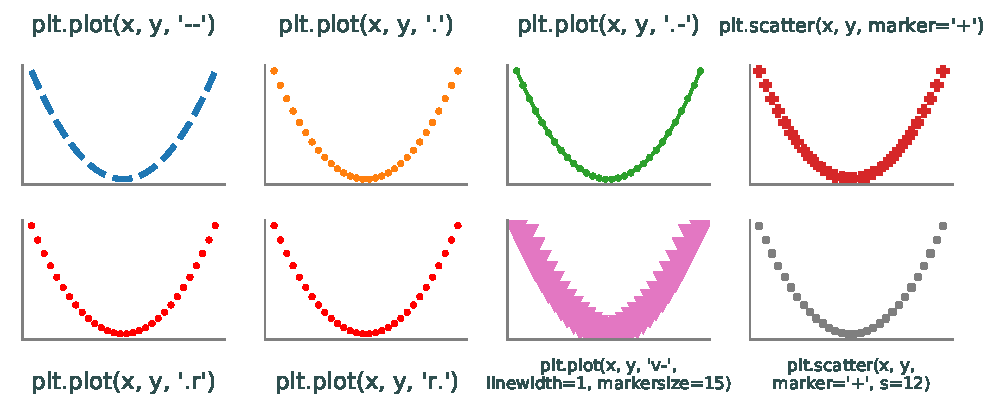
\includegraphics[width=\textwidth]{figures/linestyles_example.pdf}
\caption{Examples of setting line and marker styles.}
\label{mpl:linestyles}
\end{figure}

\section*{Plot Types} %=======================================
Matplotlib has functions for creaing many different types of plots, many of which are listed in Table \ref{mpl:plotfunctions}.
This section gives details on using certain groups of these functions.

\begin{table}[H] % Different plotting commands.
\centering
\begin{tabular}{l|p{8cm}|p{4cm}}
    Function & Description & Usage\\
    \hline
    \li{bar} & makes a bar graph & bar(x,height)\\
    \li{barh} & makes a horizontal bar graph & barh(y,width)\\
    \li{boxplots} & makes one or more boxplots & boxplots(data) \\
    \li{contour} & makes a contour plot & contour(X,Y,Z)\\
    \li{contourf} & makes a filled contour plot & contourf(X,Y,Z)\\
    \li{imshow} & shows an image & imshow(image) \\
    \li{fill} & plots lines with shading under the curve & fill(x,y)\\
    \li{fill\_between} & plots lines with shading between two given y
    values & fill\_between(x,y1, y2=0)\\
    \li{hexbin} & creates a hexbin plot & hexbin(x,y)\\
    \li{hist} & plots a histogram from data & hist(data)\\
    \li{pcolormesh} & makes a heatmap & pcolormesh(X,Y,Z) \\
    \li{pie} & makes a pie chart & pie(x)\\
    \li{plot} & plots lines and data on standard axes & plot(x,y)\\
    \li{plot_surface} & plot a surface in 3-D space & plot\_surface(X,Y,Z)\\
    \li{polar} & plots lines and data on polar axes & polar(theta,r)\\
    \li{loglog} & plots lines and data on logarithmic x and y axes &
    loglog(x,y)\\
    \li{scatter} & plots data in a scatterplot & scatter(x,y)\\
    \li{semilogx} & plots lines and data with a log scaled x axis &
    semilogx(x,y)\\
    \li{semilogy} & plots lines and data with a log scaled y axis &
    semilogy(x,y)\\
    \li{specgram} & makes a spectogram from data & specgram(x)\\
    \li{spy} & plots the sparsity pattern of a 2D array & spy(Z)\\
    \li{triplot} & plots triangulation between given points &
    triplot(x,y)\\
\end{tabular}
\caption{Some basic plotting functions in Matplotlib.}
\label{mpl:plotfunctions}
\end{table}

\subsection*{Line plots}
Line plots, the most basic type of plot, are created with the \li{plot()} function.
It accepts two lists of x- and y-values to plot, and optionally a third argument of a string of any combination of the color, line style, and marker style.
Note that this method only works with the single-character color codes; to use other colors, use the \li{color} argument.
By specifying only a marker style, this function can also be used to create scatterplots.

There are a number of functions that do essentially the same thing as \li{plot()} but also change the axis scaling, including \li{loglog()}, \li{semilogx()}, \li{semilogy()}, and \li{polar}.
Each of these functions is used in the same manner as \li{plot()}, and has identical syntax.

\subsection*{Bar Plots}
Bar plots are a way to graph categorical data in an effective way. They are made using the \li{bar()} function. The most important arguments are the first two that provide the data, \li{x} and \li{height}. The first argument is a list of values for each bar, either categorical or numerical; the second argument is a list of numerical values corresponding to the height of each bar. There are other parameters that may be included as well. The \li{width} argument adjusts the bar widths; this can be done by choosing a single value for all of the bars, or an array to give each bar a unique width. Further, the argument \li{bottom} allows one to specify where each bar begins on the y-axis. Lastly, the \li{align} argument can be set to 'center' or 'edge' to align as desired on the x-axis. As with all plots, you can use the \li{color} keyword to specify any color of your choice. 
If you desire to make a horizontal bar graph, the syntax follows similarly using the function \li{barh()}, but with argument names \li{y}, \li{width}, \li{height} and \li{align}.

\subsection*{Box Plots}
A box plot is a way to visualize some simple statistics of a dataset. It plots the minimum, maximum, and median along with the first and third quartiles of the data. This is done by using \li{boxplot()} with an array of data as the argument. Matplotlib allows you to enter either a one dimensional array for a single box plot, or a 2-dimensional array where it will plot a box plot for each column of the data in the array. Box plots default to having a vertical orientation but can be easily laid out horizontally by setting \li{vert=False}.

\subsection*{Scatter and hexbin plots}
Scatterplots can be created using either \li{plot()} or \li{scatter()}.
Generally, it is simpler to use \li{plot()}, although there are some cases where  \li{scatter()} is better.
In particular, \li{scatter()} allows changing the color and size of individual points within a single call to the function.
This is done by passing a list of colors or sizes to the \li{c} or \li{s} arguments, respectively.

Hexbin plots are an alternative to scatterplots that show the concentration of data in regions rather than the individual points.
They can be created with the function \li{hexbin()}.
Like \li{plot()} and \li{scatter()}, this function accepts two lists of x- and y-coordinates.

%The following example demonstrates using \li{scatter()} and \li{hexbin()}.
%The results is shown in Figure \ref{mpl:contour}
%\begin{lstlisting}
%\end{lstlisting}
%\begin{figure}[H]
%\centering
%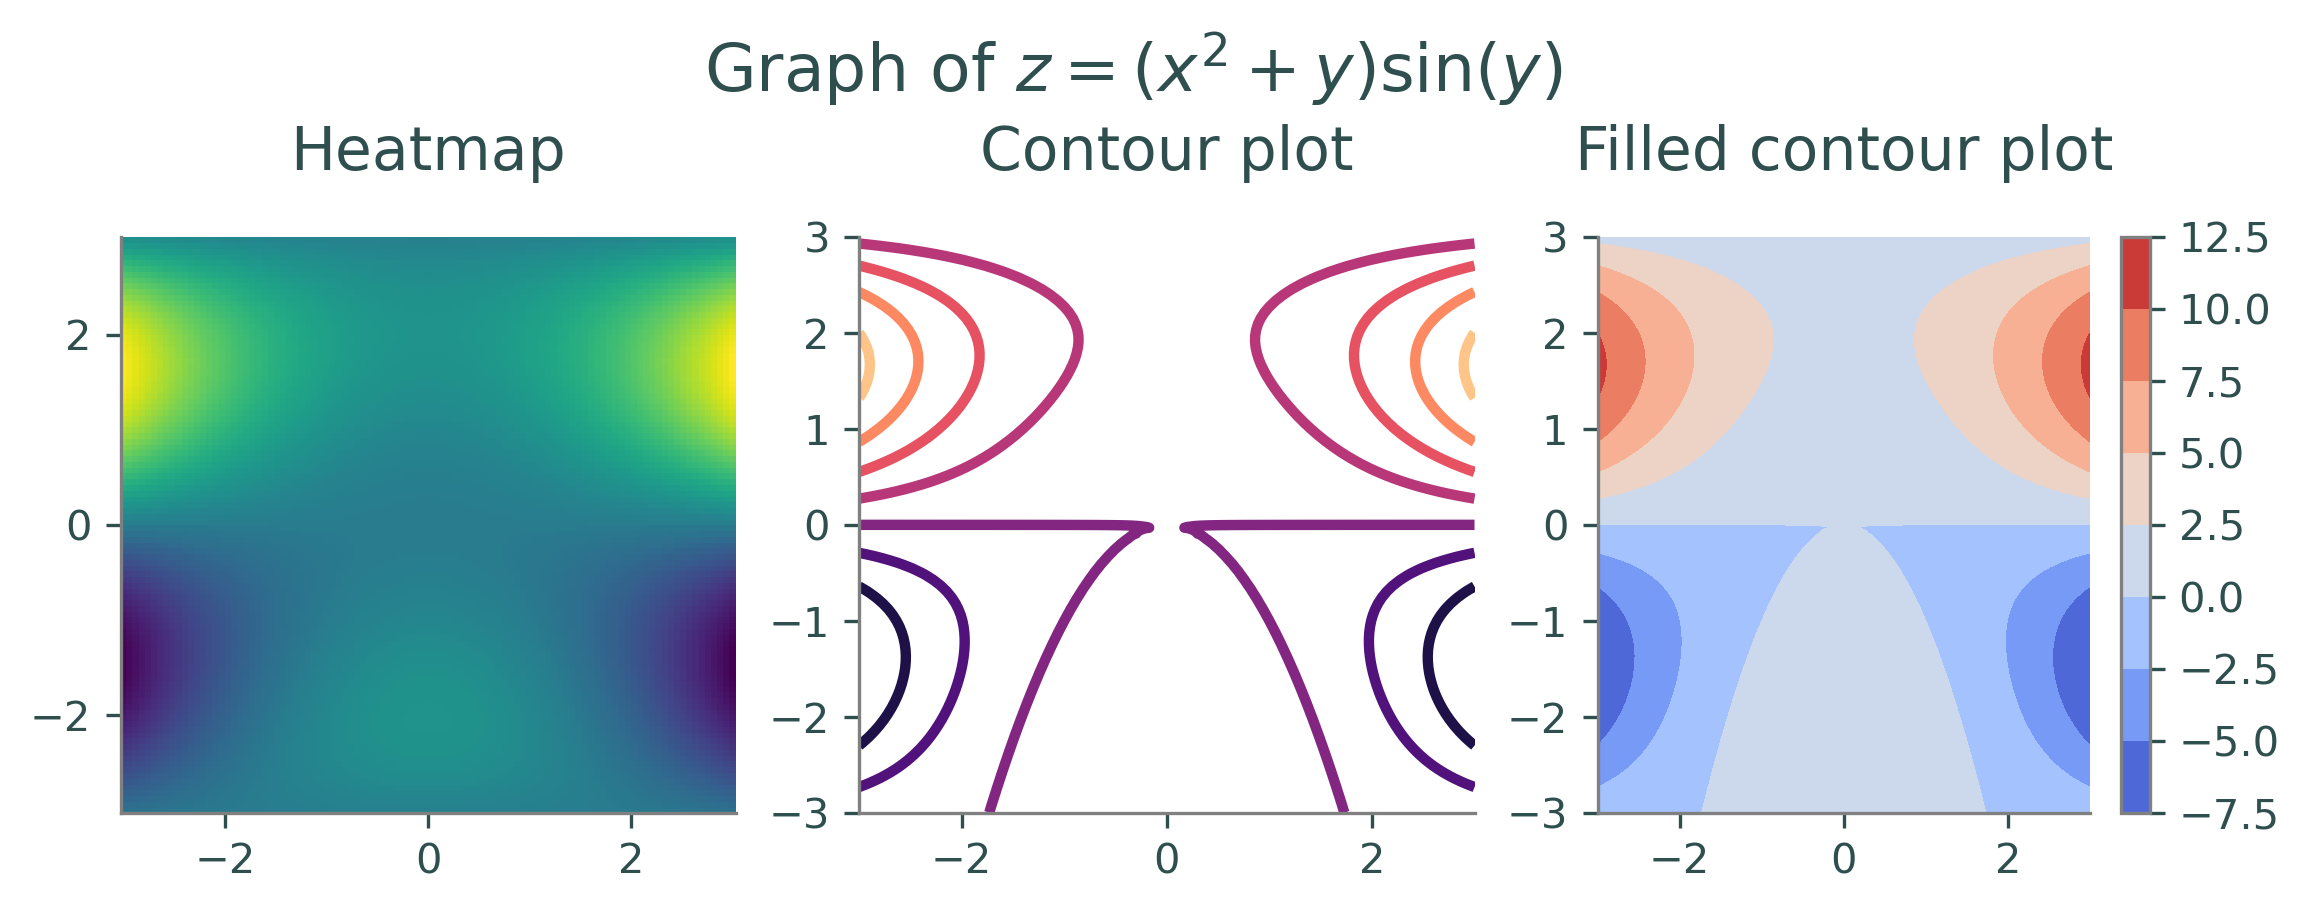
\includegraphics[width=\textwidth]{figures/heat_contour_example.pdf}
%\caption{Example of heatmaps and contour plots.}
%\label{mpl:contour}
%\end{figure}

\subsection*{Heatmaps and contour plots}
Heatmaps and contour plots are used to visualize 3-D surfaces and complex-valued functions on a flat space.
Heatmaps are created using the \li{pcolormesh()} function.
Contour plots are created using \li{contour()} or \li{contourf()}, with the latter creating a filled contour plot.

Each of these functions accepts the x-, y-, and z-coordinates as a mesh grid, or 2-D array.
To create these, use the function \li{np.meshgrid()}:
\begin{lstlisting}
>>> x = np.linspace(0,1,100)
>>> y = np.linspace(0,1,80)
>>> X, Y = np.meshgrid(x, y)
\end{lstlisting} 
The z-coordinate can then be computed using the x and y mesh grids.

Note that each of these functions can accept a colormap, using the \li{cmap} parameter.
These plots are sometimes more informative with a logarithmic color scale, which can be used by passing a \li{matplotlib.colors.LogNorm} object in the \li{norm} parameter of these functions.

With \li{pcolormesh()}, it is also necessary to pass \li{shading='auto'} or \li{shading='nearest'} to avoid a deprecation error.

The following example demonstrates creating heatmaps and contour plots, using a graph of $z=(x^2+y)\sin(y)$.
The results is shown in Figure \ref{mpl:contour}
\begin{lstlisting}
>>> from matplotlib.colors import LogNorm

>>> x = np.linspace(-3,3,100)
>>> y = np.linspace(-3,3,100)
>>> X, Y = np.meshgrid(x, y)
>>> Z = (X**2+Y)*np.sin(Y)

#Heatmap
>>> plt.subplot(1,3,1)
>>> plt.pcolormesh(X, Y, Z, cmap='viridis', shading='nearest')
>>> plt.title("Heatmap")

#Contour
>>> plt.subplot(1,3,2)
>>> plt.contour(X, Y, Z, cmap='magma')
>>> plt.title("Contour plot")

#Filled contour
>>> plt.subplot(1,3,3)
>>> plt.contourf(X, Y, Z, cmap='coolwarm')
>>> plt.title("Filled contour plot")
>>> plt.colorbar()

>>> plt.show()

\end{lstlisting}
\begin{figure}[H]
\centering
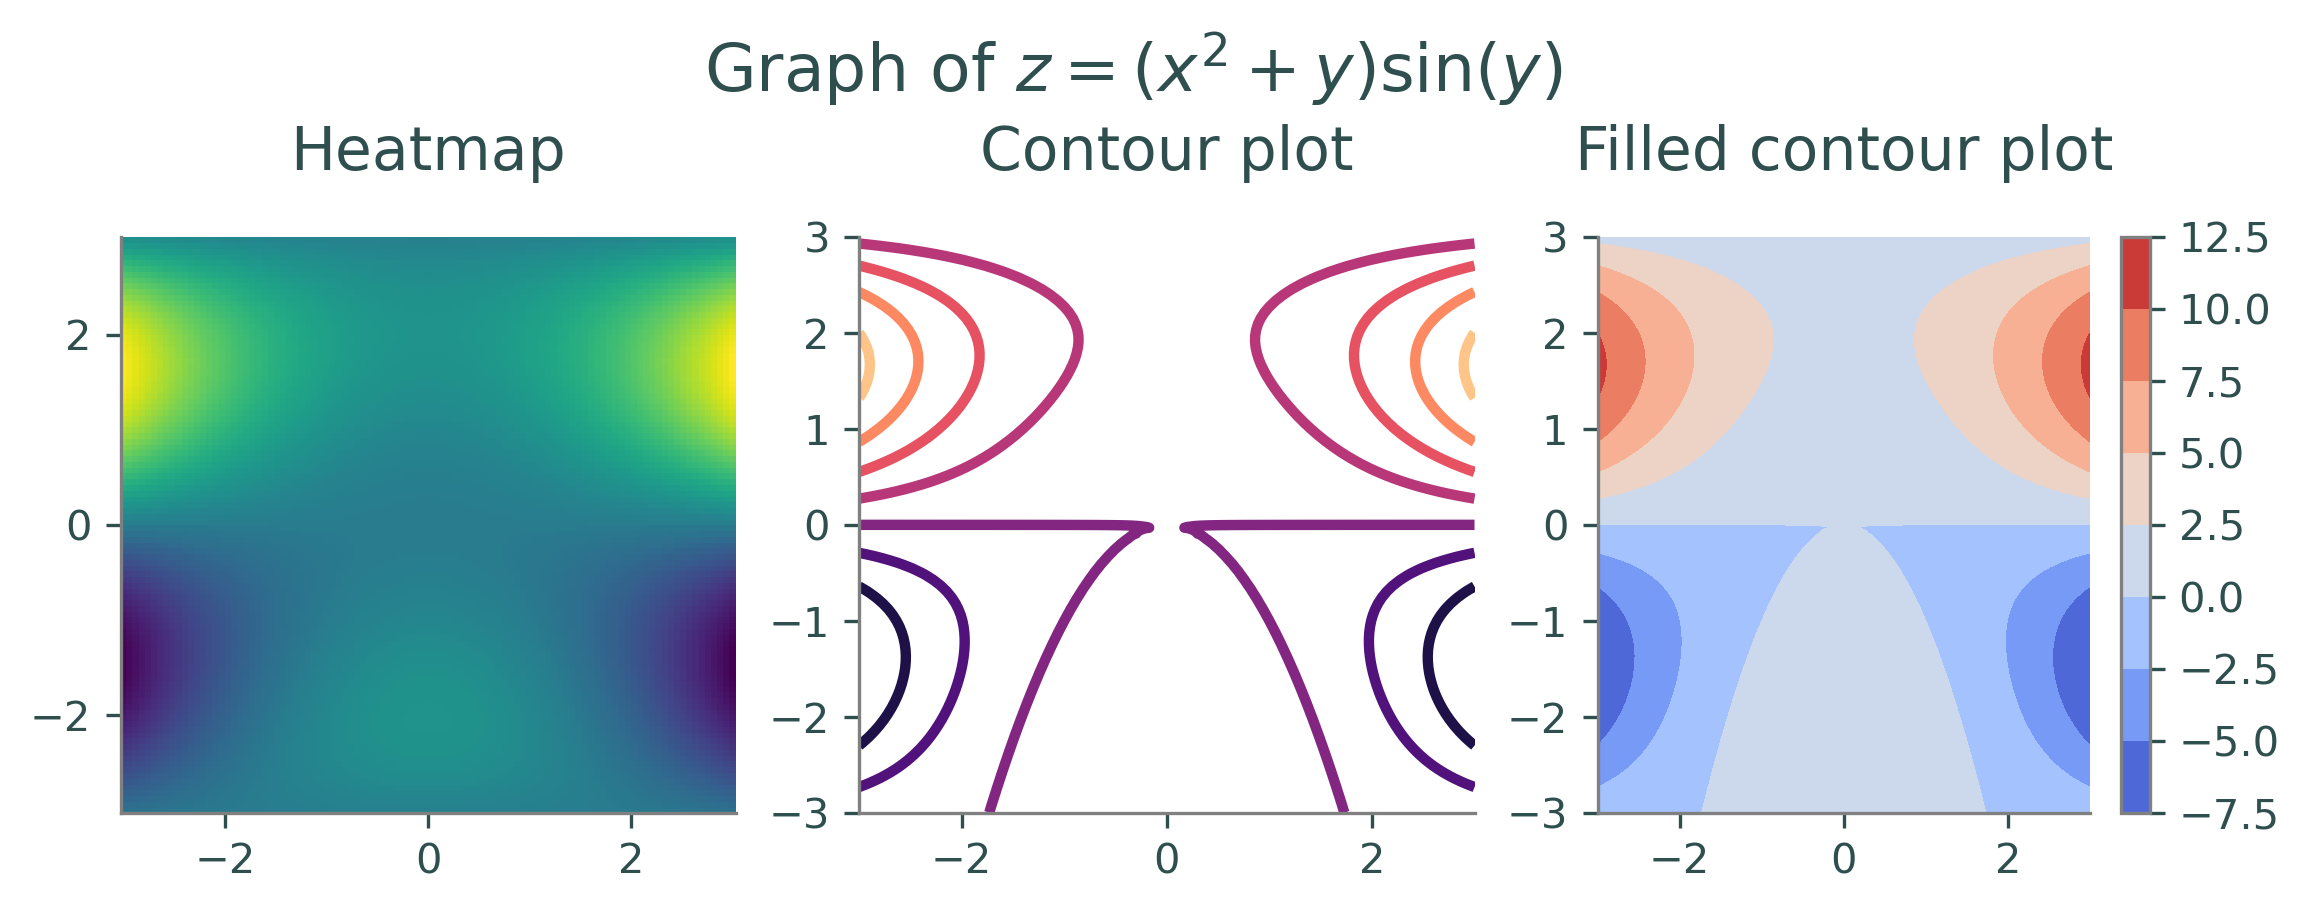
\includegraphics[width=\textwidth]{figures/heat_contour_example.png}
\caption{Example of heatmaps and contour plots.}
\label{mpl:contour}
\end{figure}

\subsection*{Showing images}
The function \li{imshow()} is used for showing an image in a plot, and can be used on either grayscale or color images.
This function accepts a 2-D $n\times m$ array for a grayscale image, or a 3-D $n\times m \times 3$ array for a color image.
If using a grayscale image, you also need to specify \li{cmap='gray'}, or it will be colored incorrectly.

It is best to also use \li{axis('equal')} alongside \li{imshow()}, or the image will most likely be stretched.
This function also works best if the images values are in the range $[0,1]$.
Some ways to load images will format their values as integers from 0 to 255, in which case the values in the image array should be scaled before using \li{imshow()}.

\subsection*{3-D Plotting}
Matplotlib can be used to plot curves and surfaces in 3-D space.
In order to use 3-D plotting, you need to run the following line:
\begin{lstlisting}
>>> from mpl_toolkits.plot3d import Axes3D
\end{lstlisting}
The argument \li{projection='3d'} also must be specified when creating the subplot for the 3-D object:
\begin{lstlisting}
>>> plt.subplot(1,1,1, projection='3d')
\end{lstlisting}

Curves can be plotted in 3-D space using \li{plot()}, by passing in three lists of x-, y-, and z-coordinates.
Surfaces can be plotted using \li{ax.plot_surface()}.
This function can be used similar to creating contour plots and heatmaps, by obtaining meshes of x- and y- coordinates from \li{np.meshgrid()} and using those to produce the z-axis.
More generally, any three 2-D arrays of meshes corresponding to x-, y-, and z-coordinates can be used.
Note that it is necessary to call this function from an Axes object.

The following example demonstrates creating 3-D plots. The results are shown in Figure \ref{mpl:3d}.

\begin{lstlisting}
#Create a plot of a parametric curve
ax = plt.subplot(1,3,1, projection='3d')
t = np.linspace(0, 4*np.pi, 160)
x = np.cos(t)
y = np.sin(t)
z = t / np.pi
plt.plot(x, y, z, color='b')
plt.title("Helix curve")

#Create a surface plot from np.meshgrid
ax = plt.subplot(1,3,2, projection='3d')
x = np.linspace(-1,1,80)
y = np.linspace(-1,1,80)
X, Y = np.meshgrid(x, y)
Z = X**2 - Y**2
ax.plot_surface(X, Y, Z, color='g')
plt.title(r"Hyperboloid")

#Create a surface plot less directly
ax = plt.subplot(1,3,3, projection='3d')
theta = np.linspace(-np.pi,np.pi,80)
rho = np.linspace(-np.pi/2,np.pi/2,40)
Theta, Rho = np.meshgrid(theta, rho)
X = np.cos(Theta) * np.cos(Rho)
Y = np.sin(Theta) * np.cos(Rho)
Z = np.sin(Rho)
ax.plot_surface(X, Y, Z, color='r')
plt.title(r"Sphere")

plt.show()
\end{lstlisting}
\begin{figure}[H]
\centering
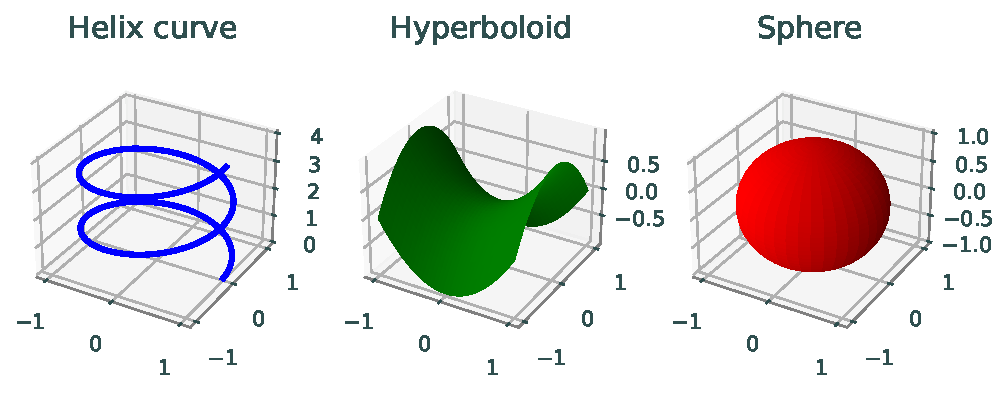
\includegraphics[width=\textwidth]{figures/3d_example.pdf}
\caption{Examples of 3-D plotting.}
\label{mpl:3d}
\end{figure}

\section*{Additional Resources} % ==============================================
\subsection*{rcParams}
The default plotting parameters of Matplotlib can be set individually and with more fine control than styles by using \li{rcParams}.
\li{rcParams} is a dictionary that can be accessed as either \li{plt.rcParams} or \li{matplotlib.rcParams}.
%technically, it isn't actually a dictionary, but just looks like one

For instance, the resolution of plots can be changed via the \li{"figure.dpi"} parameter:
\begin{lstlisting}
>>> plt.rcParams["figure.dpi"] = 600
\end{lstlisting}

A list of parameters that can set via \li{rcParams} can be found at \url{https://matplotlib.org/stable/api/matplotlib_configuration_api.html#matplotlib.RcParams}.

\subsection*{Animations}
Matplotlib has capabilities for creating animated plots.
The Animations lab in Volume 4 has detailed instructions on how to do so.

\subsection*{Matplotlib gallery and tutorials}
The Matplotlib documentation has a number of tutorials, found at \url{https://matplotlib.org/stable/tutorials/index.html}.
It also has a large gallery of examples, found at \url{https://matplotlib.org/stable/gallery/index.html}.
Both of these are excellent sources of additional information about ways to use and customize Matplotlib.


